%%%%%%%%%%%%%%%%%%%%%%%%%%%%%%%%%%%%%%%%%%%%%%%%%%%%%%%%%%%%%%%%%%
%%%%%%%%%%%%%%%%%%%%%%%%%%%%%%%%%%%%%%%%%%%%%%%%%%%%%%%%%%%%%%%%%%
%Packages
\documentclass[10pt, a4paper]{article}
\usepackage[UTF8]{ctex}
\usepackage[top=3cm, bottom=4cm, left=3.5cm, right=3.5cm]{geometry}
\usepackage{amsmath,amsthm,amsfonts,amssymb,amscd, fancyhdr, color, comment, graphicx, environ}
\usepackage{float}
\usepackage{mathrsfs}
\usepackage[math-style=ISO]{unicode-math}
\setmathfont{TeX Gyre Termes Math}
\usepackage{lastpage}
\usepackage[dvipsnames]{xcolor}
\usepackage[framemethod=TikZ]{mdframed}
\usepackage{enumerate}
\usepackage[shortlabels]{enumitem}
\usepackage{fancyhdr}
\usepackage{indentfirst}
\usepackage{listings}
\usepackage{sectsty}
\usepackage{thmtools}
\usepackage{shadethm}
\usepackage{hyperref}
\usepackage{CJKfntef}
\usepackage{setspace}
\hypersetup{
    colorlinks=true,
    linkcolor=blue,
    filecolor=magenta,      
    urlcolor=blue,
}
%%%%%%%%%%%%%%%%%%%%%%%%%%%%%%%%%%%%%%%%%%%%%%%%%%%%%%%%%%%%%%%%%%
%%%%%%%%%%%%%%%%%%%%%%%%%%%%%%%%%%%%%%%%%%%%%%%%%%%%%%%%%%%%%%%%%%
%Environment setup
\mdfsetup{skipabove=\topskip,skipbelow=\topskip}
\newrobustcmd\ExampleText{%
An \textit{inhomogeneous linear} differential equation has the form
\begin{align}
L[v ] = f,
\end{align}
where $L$ is a linear differential operator, $v$ is the dependent
variable, and $f$ is a given non−zero function of the independent
variables alone.
}
\mdfdefinestyle{theoremstyle}{%
linecolor=black,linewidth=1pt,%
frametitlerule=true,%
frametitlebackgroundcolor=gray!20,
innertopmargin=\topskip,
}
\mdtheorem[style=theoremstyle]{Problem}{作业题}
\newenvironment{Solution}{}

%%%%%%%%%%%%%%%%%%%%%%%%%%%%%%%%%%%%%%%%%%%%%%%%%%%%%%%%%%%%%%%%%%
%%%%%%%%%%%%%%%%%%%%%%%%%%%%%%%%%%%%%%%%%%%%%%%%%%%%%%%%%%%%%%%%%%
%Fill in the appropriate information below
\newcommand{\norm}[1]{\left\lVert#1\right\rVert}     
\newcommand\course{最优化方法}                         % <-- course name   
%\newcommand\hwnumber{1}                              % <-- homework number
\newcommand\Information{李邹/人工智能一班}          % <-- personal information
%%%%%%%%%%%%%%%%%%%%%%%%%%%%%%%%%%%%%%%%%%%%%%%%%%%%%%%%%%%%%%%%%%
%%%%%%%%%%%%%%%%%%%%%%%%%%%%%%%%%%%%%%%%%%%%%%%%%%%%%%%%%%%%%%%%%%
%Page setup
\pagestyle{fancy}
\headheight 35pt
\lhead{\today}
\rhead{
\includegraphics[width=2.5cm]{lzu-logo.png}}
\lfoot{}
\pagenumbering{arabic}
\cfoot{\small\thepage}
\rfoot{}
\headsep 1.2em
\renewcommand{\baselinestretch}{1.25}
%%%%%%%%%%%%%%%%%%%%%%%%%%%%%%%%%%%%%%%%%%%%%%%%%%%%%%%%%%%%%%%%%%
%%%%%%%%%%%%%%%%%%%%%%%%%%%%%%%%%%%%%%%%%%%%%%%%%%%%%%%%%%%%%%%%%%
%Add new commands here
\renewcommand{\labelenumi}{\alph{enumi})}
\newcommand{\Z}{\mathbb Z}
\newcommand{\R}{\mathbb R}
\newcommand{\Q}{\mathbb Q}
\newcommand{\NN}{\mathbb N}
\DeclareMathOperator{\Mod}{Mod} 
\renewcommand\lstlistingname{Algorithm}
\renewcommand\lstlistlistingname{Algorithms}
\def\lstlistingautorefname{Alg.}
%%%%%%%%%%%%%%%%%%%%%%%%%%%%%%%%%%%%%%%%%%%%%%%%%%%%%%%%%%%%%%%%%%
%%%%%%%%%%%%%%%%%%%%%%%%%%%%%%%%%%%%%%%%%%%%%%%%%%%%%%%%%%%%%%%%%%
%Begin now!



\begin{document}

\begin{titlepage}
    \begin{center}
        \vspace*{3.5cm}
            
        \Huge
        \textbf{作业6}
            
        \vspace{2cm}
        \LARGE
        李邹
            
        \vspace{0.1cm}
        \Large
        人工智能一班(2020级)                      % <-- author
        
            
        \vfill
        
        \course \ 课程作业
            
        \vspace{1cm}
            
        
\includegraphics[width=0.4\textwidth]{lzu-logo.png}
        \\
        
        \Large
        
        \today
            
    \end{center}
\end{titlepage}

%%%%%%%%%%%%%%%%%%%%%%%%%%%%%%%%%%%%%%%%%%%%%%%%%%%%%%%%%%%%%%%%%%
%%%%%%%%%%%%%%%%%%%%%%%%%%%%%%%%%%%%%%%%%%%%%%%%%%%%%%%%%%%%%%%%%%
%Start the assignment now

%%%%%%%%%%%%%%%%%%%%%%%%%%%%%%%%%%%%%%%%%%%%%%%%%%%%%%%%%%%%%%%%%%
%New problem
\newpage
\begin{Problem}
假设$f:R\longrightarrow R$是凸函数,$a,b\in \textbf{dom}\,f,a<b,$
\begin{enumerate}[(a)]
	\item 证明对任意$x\in \left [ a,b \right ] $,下式成立
    \[f\left ( x \right ) \le \frac{b-x}{b-a} \, f\left ( a \right ) +\frac{x-a}{b-a} \, f\left ( b \right ) \]
	\item 证明对任意$x\in \left ( a,b \right ) $,下式成立
    \[\frac{f(x)-f(a)}{x-a} \le \frac{f(b)-f(a)}{b-a}\le \frac{f(b)-f(x)}{b-x}  \]
    画一个草图来描述此不等式。
	\item 假设函数$f$可微。利用$(b)$中的结果来证明
    \[f^{\prime}(a) \leq \frac{f(b)-f(a)}{b-a} \leq f^{\prime}(b)\]
    注意到这些不等式也可以通过$(3.2)$得到:
    \[f(b) \geq f(a)+f^{\prime}(a)(b-a)\]\[f(a) \geq f(b)+f^{\prime}(b)(a-b)\]
	\item 假设函数$f$二次可微。利用$(c)$中的结论证明$f^{''}(a)\ge 0 $以及$f^{''}(b)\ge 0$。
\end{enumerate}
\end{Problem}
    
\begin{Solution}
\textbf{证明}
\end{Solution}
%%%%%%%%%%%%%%%%%%%%%%%%%%%%%%%%%%%%%%%%%%%%%%%%%%%%%%%%%%%%%%%%%%
%Complete the assignment now
\begin{enumerate}[(a)]
	\item 由题,$f$是凸函数,$a,b\in \textbf{dom}\,f $,则有,
    \begin{align}
        f(\theta a+(1-\theta) b) \leq \theta f(a)+(1-\theta) f(b) \label{1}
    \end{align}

    令$\theta = \frac{b-x}{b-a} $,由于$a<b$,则$\theta\in  \left [ 0,1 \right ] $一定成立。\\\\
    代入(\ref*{1})式,则有,\[f\left(\frac{b-x}{b-a} a+\frac{x-a}{b-a} b\right)=f(x)\le \frac{b-x}{b-a}\, f(a)+\frac{x-a}{b-a}\, f(b)\]
    \hfill $\Box$ 

	\item 将(\ref*{1})式去分母化,得
    \begin{align}
        &(b-a) f(x) \leq(b-x)\, f(a)+(x-a)\, f(b) \notag   \\
        \Longleftrightarrow&(b-a) f(x)-(b-a) f(a) \leq(a-x) f(a)+(x-a) f(b) \notag \\
        \Longleftrightarrow&\frac{f(x)-f(a)}{x-a} \leq \frac{f(b)-f(a)}{b-a} \label{2}
    \end{align}
    同理可得:
    \begin{align}
        &(b-a) f(x)-(b-a) f(b) \leq(b-x) f(a)+(x-b) f(b)   \notag \\
        \Longleftrightarrow&\frac{f(b)-f(x)}{b-x} \leq \frac{f(b)-f(a)}{b-a} \label{3}
    \end{align}
    合并(\ref*{2})(\ref*{3})式,即得,\[\frac{f(x)-f(a)}{x-a} \le \frac{f(b)-f(a)}{b-a}\le \frac{f(b)-f(x)}{b-x}  \]
    \begin{figure}[h]
        \centering
        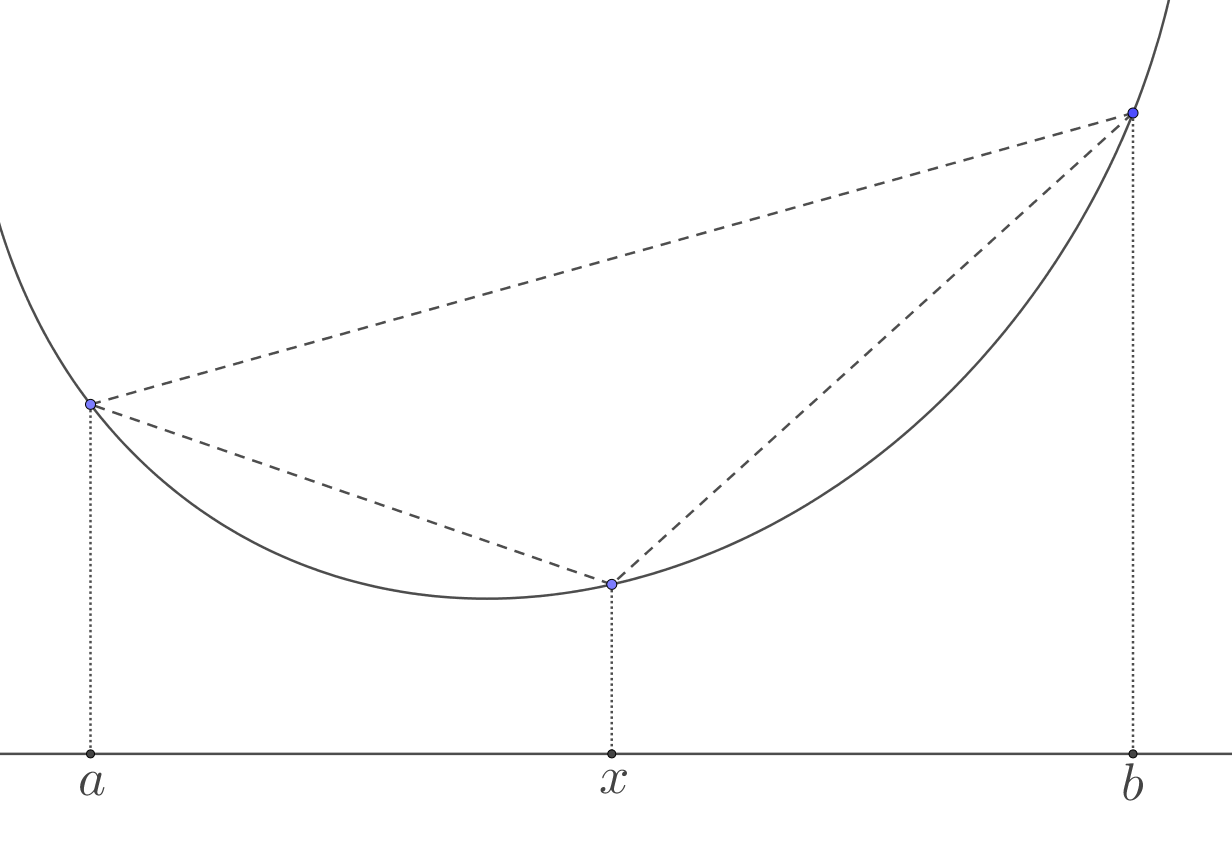
\includegraphics[scale=0.22]{t2.png}
        \caption{描述(b)中不等式的草图}
    \end{figure}    
    \hfill $\Box$

	\item 当$x\to a$时,由微分的定义,有
    \begin{align}
        \frac{f(x)-f(a)}{x-a} & = f^{\prime}(a) \notag
    \end{align}
    代入(\ref*{2})式,有
    \begin{align}
        f^{\prime}(a) \leq \frac{f(b)-f(a)}{b-a}    \label{4}
    \end{align}
    同理可得:
    \begin{align}
        \frac{f(b)-f(a)}{b-a} \leq f^{\prime}(b)    \label{5}
    \end{align}
    综合(\ref*{4})(\ref*{5})式,可得
    \begin{align}
        f^{\prime}(a) \leq \frac{f(b)-f(a)}{b-a} \leq f^{\prime}(b) \label{6}
    \end{align}
    \hfill $\Box$

	\item 由(\ref*{6})有$f^{\prime}(a) \leq f^{\prime}(b)$,由于$a<b$,则有:
    \begin{align}
        \frac{f^{\prime}(b)-f^{\prime}(a)}{b-a} \geq 0  \label{7}
    \end{align}
    当$a\to b$时,(\ref*{7})式可化为:
    \begin{align}
        f^{\prime \prime}(b) \geq 0 \notag
    \end{align}
    同理可得:
    \begin{align}
        f^{\prime \prime}(a) \geq 0 \notag
    \end{align}
    \hfill $\Box$
\end{enumerate}
\vspace*{3em}
\begin{Problem}
推导下列函数的共轭函数
\begin{enumerate}[(a)]
	\item \textbf{最大值函数}。函数$\max_{i=1,\dots ,n} x_{i} $,定义在$\mathbf{R}^{n} $上。
	\item \textbf{最大若干分量之和}。函数$f(x)=\sum_{i=1}^{r} x_{[i]}$,定义域为$\mathbf{R}^{n} $。
	\item \textbf{定义在$R$上的线性分片函数}。定义在$\mathbf{R}$上的线性分片函数$f(x)=\max _{i=1, \ldots, m}(a_{i} x+$\\$b_{i})$。在求解过程中,可以假设$a_{i} $按升序排列,即$a_{1} \leq \cdots \leq a_{m}$,且每一个函数$a_{i} x+b_{i}$都不是冗余的,即任选$k$,至少存在一点$x$使得$f(x)=a_{k}x+b_{k}  $。
	\item \textbf{幂函数}。定义在$\mathbf{R}_{++} $上的函数$f(x)=x^{p} $,其中$p>1$。如果$p<0$呢?
    \item \textbf{几何平均}。定义在$\mathbf{R}_{++}^{n} $上的几何平均函数$f(x)=-\left(\prod x_{i}\right)^{1 / n}$。
    \item \textbf{二阶锥上的负广义对数}。函数$f(x, t)=-\log \left(t^{2}-x^{T} x\right)$,定义域为$\{(x, t) \in \mathbf{R}^{n} \times \mathbf{R} \mid\|x\|_{2}<t\}$。
\end{enumerate}
\end{Problem}

\begin{Solution}
\textbf{解答}
\end{Solution}

\begin{enumerate}[(a)]
	\item 由定义有,
    \begin{align}
        f^{*}(y) & = \sup _{x}\left\{y^{T} x-\max x\right\}     \notag
    \end{align}
    首先考虑$y$分量中是否存在负值,若存在负值,则对应的$x^{T} \to \infty $时,函数无上界,因此$y\succeq 0$必然成立。其次考虑$y$是否存在大于1的分量,若存在,则对应的$x_{i} \to \infty $时,函数无上界,因此$y\preceq 1$必然成立。\\
    \\综上,我们将定义域限制在$0\preceq y\preceq 1$的范围中。\\设$x \in \mathbf{R}^{n}$的各分量按从大到小排序为$x_{1} \geq x_{2} \geq \cdots \geq x_{n}$\\
    于是有:\[f^{*}(y) = \sup _{x}\left\{\sum_{i = 1}^{n} y_{i} x_{i}-x_{1}\right\} = \sup _{x}\left\{\left(y_{1}-1\right) x_{1}+\sum_{i = 2}^{n} y_{i} x_{i}\right\}, \quad \forall i \geq 2 \quad x_{i} \leq x_{1}\]
    考虑使函数逼近上界的$x$取值,不妨取各个分量相等的向量,即$x= t\textbf{1} $,则有:
    \[f^{*}(y)=\sup _{x}\left\{\left(y_{1}-1\right) x_{1}+\sum_{i=2}^{n} y_{i} x_{i}\right\}=\sup _{t}\left\{t\left(\sum_{i=1}^{m} y_{i}-1\right)\right\}\]
    容易发现,当且仅当$\sum_{i} y_{i}=1$时,函数值才不受变量$t$的控制,上界一定存在。\\
    此时,\[f^{*}(y) = 0\]
    综上所述:
    \[f^{*}(y) = \left\{\begin{array}{ll}
        0 & \text { if } y \succeq 0, \quad \mathbf{1}^{T} y = 1 \\
        \infty & \text { otherwise }
        \end{array}\right.\]

	\item 与(a)类似,不难确定本小问的定义域为$0\preceq y\preceq 1$\\
    设$x \in \mathbf{R}^{n}$的各分量按从大到小排序为$x_{1} \geq x_{2} \geq \cdots \geq x_{n}$\\
    于是有:\[f^{*}(y)=\sup \left\{\sum_{i=1}^{r}\left(y_{i}-1\right) x_{i}+\sum_{i=r+1}^{n} y_{i} x_{i}\right\}\]
    考虑最大化函数值的$x$取值,不妨取各个分量相等的向量,即$x= t\textbf{1} $,则有:
    \[f^{*}(y)=\sup \left\{\sum_{i=1}^{r}\left(y_{i}-1\right) x_{i}+\sum_{i=2}^{n} y_{i} x_{i}\right\}=\sup \left\{t\left(\sum_{i=1}^{m} y_{i}-r\right)\right\}\]
    容易发现,当且仅当$\sum_{i} y_{i}=r$时,函数值才不受变量$t$的控制,上界一定存在。\\
    此时,\[f^{*}(y) = 0\]
    综上所述:
    \[f^{*}(y)=\left\{\begin{array}{ll}
        0 & \text { if } \quad 0 \preceq y \preceq 1, \quad \mathbf{1}^{\mathbf{T}} y=r \\
        \infty & \text { otherwise }
        \end{array}\right.\]
    
	\item 对于$f(x)=\max _{i=1, \ldots, m}(a_{i} x+b_{i})$,存在$m-1$个拐点,其表达式为:
    \[x_{i}=\frac{b_{i}-b_{i+1}}{a_{i+1}-a_{i}}, \quad i=1, \ldots, m-1\]
    因此,不难求得:
    \[f^{*}(y)=-b_{i}-\frac{b_{i+1}-b_{i}}{a_{i+1}-a_{i}}\left(y-a_{i}\right)\]
    其中,$y \in\left[a_{i}, a_{i+1}\right]$

	\item \textbf{先考虑$p>1$的情况}\\
    由$y=\nabla f(x)=p x^{p-1} $可得:
    \begin{align}
        x & = \left(\frac{y}{p}\right)^{\frac{1}{p-1}} \label{8}
    \end{align}
    当$y>0$时,将(\ref*{8})式代入共轭函数定义式中,则有:
    \begin{align}
        f^{*}(y) & = y\left(\frac{y}{p}\right)^{\frac{1}{p-1}}-\left(\frac{y}{p}\right)^{\frac{p}{p-1}} \notag \\
        & = (p-1)\left(\frac{y}{p}\right)^{\frac{p}{p-1}} \notag
    \end{align}
    当$y\le 0$时,显然有$f^{*}(y)=0$.
    综上所述:
    \[f^{*}(y)=\left\{\begin{array}{ll}
        0 & y \leq 0 \\
        (p-1)\left(\frac{y}{p}\right)^{\frac{p}{p-1}} & y>0
        \end{array}\right.\]
    \textbf{再考虑$p<0$的情况}\\
    此时定义域变换为$-\mathrm {R}_{++} $,同理可得:
    \begin{align}
        f^{*}(y) & = -y\left(\frac{-y}{p}\right)^{\frac{1}{p-1}}+\left(\frac{-y}{p}\right)^{\frac{p}{p-1}} \notag \\
        & = (1-p)\left(\frac{-y}{p}\right)^{\frac{p}{p-1}}  \notag
    \end{align}

    \item 假设$y$中存在一个大于0的分量,设其为$y_{k}>0$\\
    令$x_{k}=t,x_{i}=1\,(i\neq k)$,当$t \to \infty$时有:
    \[f^{*}(y)=t y_{k}+t^{\frac{1}{n}} \to \infty\]
    因此,$y\notin \textbf{dom}\; f$\\
    当$y$中不存在一个大于0的分量,且$\left(\prod_{i}\left(-y_{i}\right)\right)^{\frac{1}{n} }<\frac{1}{n} $时。\\
    不妨取$x=-\frac{t}{y}$,且$t \to \infty$,则有:
    \[f^{*}(y)=-\operatorname{tn}-t\left(\prod_{i}\left(-\frac{1}{y_{i}}\right)\right)^{\frac{1}{n}}>t \rightarrow \infty\]
    此时,同样有$y\notin \textbf{dom}\; f$\\
    当$y$中不存在一个大于0的分量,且$\left(\prod_{i}\left(-y_{i}\right)\right)^{\frac{1}{n} }\ge \frac{1}{n} $时,则有:
    \[x^{T} y=\sum_{i=1}^{n} x_{i} y_{i} \leq-n\left(\prod_{i=1}^{n}-x_{i} y_{i}\right)^{\frac{1}{n}} \leq-n \cdot  \frac{1}{n}\left(\prod_{i=1}^{n} x_{i}\right)^{\frac{1}{n}}=f(x)\]
    从而有
    \[f^{*}(y)=x^{T} y-f(x) \leq 0\]
    综上所述,$f^{*}(y)=0$

    \item 分两种情况讨论。\\
    \textbf{当$\|y\|_{2} \geq u$时}\\
    不妨取$x=s y\,,\, t=s\left(\|y\|_{2}+1\right)>s u\,,\,s \to \infty$,则有:
    \[x^{T} y+t u+\log \left(t^{2}-x^{T} x\right)>s u^{2}+s u^{2}+\log \left(s^{2}\right) \rightarrow \infty\]
    上界不存在,因此$y\notin \textbf{dom}\; f$\\
    \textbf{当$\|y\|_{2} < u$时}\\
    此时$(y, u)=\nabla f(x, t), f(x, t)=-\log \left(t^{2}-x^{T} x\right)$,计算可得:
    \[u=-\frac{2 t}{t^{2}-x^{T} x}, y=\frac{2 x}{t^{2}-x^{T} x}\]
    下面尝试反解出$x,t$,不难得到:
    \begin{align}
        x = \frac{2 y}{u^{2}-y^{T} y}, t = -\frac{2 u}{u^{2}-y^{T} y} \label{9}
    \end{align}
    将(\ref*{9})式代入$g(y,u)$中,即得:
    \begin{align}
        g(y, u) & = x^{T} y+t u+\log \left(t^{2}-x^{T} x\right) \notag \\
        & = -2+\log \left(\frac{4}{u^{2}-y^{T} y}\right) \notag
    \end{align}

\end{enumerate}

\begin{center}
    \fbox
    {\shortstack[l]{
      \textbf{注}\; 在《Convex Optimization Solutions Manual》中,编者给出本小问的参考答案为\\
      $2+\log 4-\log \left(y^{2}-u^{t} u\right)$,显然$y$不应为平方的形式,而应当以转置相乘的形式参与运算。\\
      值得注意的是,参考答案中$y^{2}-u^{t} u$似乎不在$log$函数所要求的定义域中。
    }}
\end{center}

\end{document}

%%%%%%%%%%%%%%%%%%%%%%%%%%%%%%%%%%%%%%%%%%%%%%%%%%%%%%%%%%%%%%%%%%
%%%%%%%%%%%%%%%%%%%%%%%%%%%%%%%%%%%%%%%%%%%%%%%%%%%%%%%%%%%%%%%%%%
